\documentclass{article}
\usepackage{amsmath,amssymb}
\usepackage{graphicx}
\usepackage[most]{tcolorbox}
\usepackage{hyperref}
\hypersetup{
  linkbordercolor={1 1 1},  % white border (RGB 1 1 1)
  pdfborder={0 0 0},
  filecolor=magenta,
  pdfpagemode=FullScreen
}
\urlstyle{same}
\usepackage{geometry}
\geometry{margin=1in}

\usepackage{enumitem}
\setlist{itemsep=5pt, topsep=5pt}
\usepackage{titlesec}
\titleformat{\section}{\normalfont\Large\bfseries\color{blue!70!black}}{}{0em}{}
\titleformat{\subsection}[runin]{\bfseries\color{blue!80!black}}{}{0em}{}[.]
\titleformat{\subsubsection}[runin]{\itshape\color{black}}{}{0em}{}[.]
\usepackage{xcolor}

\title{\textbf{Calculus BC Scrapbook: Chapter 10 – Infinite Sequences and Series}}
\author{
  Thavas Antonio\\
  \small\href{https://github.com/BuddyBob/Chapter10}{Chapter 10 GitHub Repository} % Assumed new repo
}
\date{May 2025} % Or current date if preferred

\begin{document}

\maketitle
\tableofcontents % This will list sections you create later in this chapter
\newpage

\section{Introduction to the Infinite!}

Chapter 10! Here we will dive into the infinite. Lets see how to express complex functions with simpler, infinite polynomials.

Key topics we'll explore include:
\begin{itemize}
    \item Understanding sequences and how they diverge or converge
    \item How to sum up an infinite list of numbers and determine if that sum is a finite value.
    \item Well look at the (Integral Test, Comparison Tests, Ratio Test, and more!) to better analyze behaviour
    \item Alternating series.
    \item Taylor and Maclaurin series something our class found fairly tricky. Helps us approximate functions. 
\end{itemize}

\medskip
\noindent
\textbf{What this scrapbook chapter does.} Just like before, each Big Idea will get its own dedicated space, usually two pages:

\begin{itemize}
  \item \textbf{Concept} We'll break down: 1. The definition. 2. A friendly explanation (How I'd want it explained to me). 3. Essential vocabulary. 4. Diagrams/visuals 5. Illustrative examples to best see what your doing.
  \item \textbf{Answer} Detailed solutions for the examples
\end{itemize}

Goal is to create a revisable guide for previously learned concepts. 

\vspace{10pt}


\begin{tcolorbox}[title=Chapter 10 Road-Map: All 15 Infinite-Series Big Ideas,
                  colback=gray!8, colframe=purple!70!black]

\begin{enumerate}[itemsep=3pt, topsep=2pt] 
  \item 10.1  Defining Convergent \& Divergent Infinite Series
  \item 10.2  Working with Geometric Series
\end{enumerate}

\end{tcolorbox}
\newpage


%==================== 10.1 Concept Page ====================
\section{10.1 Defining Convergent \& Divergent Infinite Series}

\begin{tcolorbox}[colback=gray!6!white,colframe=gray!60!gray,
                  title=Big-Idea: Converging]
Given an infinite series
\[
\sum_{n=1}^{\infty} a_n \;=\; a_1 + a_2 + a_3 + \dots,
\]

\begin{minipage}{0.48\linewidth}
\begin{tcolorbox}[colback=white] 
\centering
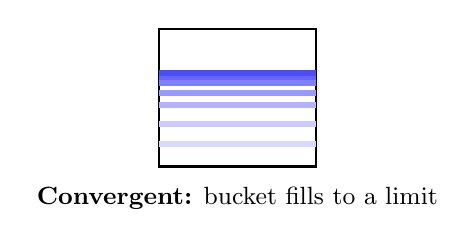
\begin{tikzpicture}[scale=0.5]
  % bucket
  \draw[thick] (0,0) rectangle (4,3.5);
  % water bars
  \foreach \h/\c in {0.5/blue!15,1/blue!20,1.5/blue!30,1.8/blue!40,2.05/blue!50,2.20/blue!60,2.30/blue!70} {
    \fill[\c] (0,\h) rectangle (4,\h+0.15);
  }
  % label
  \node at (2,-0.8) {\small \textbf{Convergent:} bucket fills to a limit};
\end{tikzpicture}
\end{tcolorbox}
\end{minipage}
\hfill
\begin{minipage}{0.48\linewidth}
\begin{tcolorbox}[colback=white] 
\centering
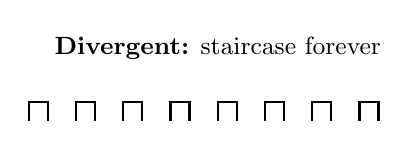
\begin{tikzpicture}[scale=0.6]
  \foreach \n in {0,1,...,7}{
    \draw[thick] (\n,0) -- (\n,0.4) -- (\n+0.4,0.4) -- (\n+0.4,0);
  }
  \node[above] at (4,1.1) {\small \textbf{Divergent:} staircase forever};
\end{tikzpicture}
\end{tcolorbox}
\end{minipage}
\end{tcolorbox}
Hopefully pretty understandable and intuitive given these diagrams.

\vspace{6pt}

\begin{tcolorbox}[colback=yellow!10,colframe=gray,title=(nth-term test)]
If \(\displaystyle\lim_{n\to\infty} a_n \neq 0\),  
then \(\sum a_n\) \emph{must} diverge.  
\end{tcolorbox}

\subsection*{Worked Mini-Examples (with extra commentary)}

\begin{enumerate}[label=\textbf{\arabic*.},topsep=4pt,itemsep=10pt]

  \item \textbf{Geometric}  
        \[
        \sum_{n=0}^{\infty}\Bigl(\tfrac13\Bigr)^{\!n}
        \]
        \begin{itemize}[itemsep=2pt]
          \item Note! The geometric with ratio \(r=\tfrac13\).
          \item Rule: a geometric series converges if \(|r|<1\).
          \item Plug \(r\) into the sum formula \(\dfrac{a}{1-r}\)  
                (here \(a=1\) when \(n=0\)):
                \[
                  S = \frac{1}{1-\tfrac13} = \frac32.
                \]
          \item I think about it like balls bouncing into a bucket where each bounce gets smaller 1/3 of the last height. 
        \end{itemize}

  % ---------- 2 ----------
  \item \textbf{Harmonic Heartbreak}  
        \[
        \sum_{n=1}^{\infty}\frac1n
        \]
        \begin{itemize}[itemsep=2pt]
          \item The terms \(\tfrac1n\) do go to \(0\) but like really slow.  
          \item It’s a \(p\)-series with \(p=1\). Remember that a \(p\)-series converges only if \(p>1\).  
        \end{itemize}

\end{enumerate}

% ---------- Quick-Check ----------
\begin{tcolorbox}[colback=green!5!white,colframe=green!50!black,title=Quick-Check]
Does \( \displaystyle\sum_{n=1}^{\infty}\frac{1}{n^{2}} \) converge? (Hint: \(p>1\).)

\begin{tcolorbox}[colback=white, sharp corners, boxrule=0pt, title=Spoiler – click to reveal, breakable]
Yes. It’s a \(p\)-series with \(p=2>1\), so it converges.  
\end{tcolorbox}
\end{tcolorbox}

\subsection*{Take-Away}
Convergence is just your partial sums calming down.  
When in doubt think “Do the terms go to zero? Which test applies?”  

 % - - - -- -- - - - - - - - 10.2  - - - - - - - - -- %
\newpage

%==================== 10.2 Working with Geometric Series ====================
\section{10.2 Working with Geometric Series}

\begin{tcolorbox}[colback=gray!10!white,colframe=gray!75!black,title=What's a Geometric Series Anyway?]
Imagine you're adding up numbers, but there's a special trick: to get the next number, you just multiply the current one by the \textbf{same value} every time. This special multiplier is called \(r\) (the common ratio).

The series looks like this:
\[
a + ar + ar^2 + ar^3 + \dots \quad \text{  }
\]
Here, \(a\) is just your \textbf{starting number}.

\textbf{Does it add up to something real (converge)?}
\begin{itemize}
    \item \textbf{YES, if \(|r| < 1\)} (meaning \(r\) is a fraction between -1 and 1, like 0.5 or -0.7).
    The sum is: \[ \boxed{S = \frac{a}{1-r}} \]
    \item \textbf{NO, if \(|r| \ge 1\)} (meaning \(r\) is 1, -1, or bigger/smaller than that). The sum just runs off to infinity or bounces around like crazy (diverges).
\end{itemize}

\end{tcolorbox}

\subsection*{Why does this \(|r|<1\) trick work?}
Think about it:
\begin{itemize}
    \item If \(r\) is small (like \(\frac{1}{2}\)), each new number you add (\(ar, ar^2, \dots\)) gets smaller and smaller. Eventually, they become so tiny they barely make a dent in the total sum. 
    \item If \(r\) is big (like 2 or -3), the numbers you add keep getting bigger. The sum never settles. 
\end{itemize}
So, that little \(r\) is the actually REALLY key!

\subsection*{Words You Might Hear}
\begin{itemize}
    \item \textbf{Geometric Series:} Our star for today – sum with a common multiplier.
    \item \textbf{Common Ratio (\(r\)):} That special number you keep multiplying by.
    \item \textbf{First Term (\(a\)):} Where your sum kicks off.
    \item \textbf{Converges:} The sum heads to a nice, single number.
    \item \textbf{Diverges:} The sum doesn't settle down (goes to infinity or bounces around).
\end{itemize}
If this looks hard to remember you eventually get the hang of it like deriv rules.

%------------------------------------------------------------
\subsection*{Let's Try Some!}

\begin{enumerate}[label=\textbf{\arabic*.},itemsep=15pt] % Increased itemsep for more space

  \item \textbf{Example 1: A Converging Friend} \\
        What about this series: \(\displaystyle\sum_{n=0}^{\infty}\left(\frac{1}{4}\right)^n = 1 + \frac{1}{4} + \frac{1}{16} + \dots\)?

        \textbf{Here's the thinking:}
        \begin{itemize}
            \item My starting number \(a\) is \((\frac{1}{4})^0 = 1\).
            \item My special multiplier \(r\) is \(\frac{1}{4}\).
            \item Is \(|r| < 1\)? Yes! \(|\frac{1}{4}| = \frac{1}{4}\), which is definitely less than 1. So, it converges!
            \item What's the sum? Use the magic formula:
                  \[ S = \frac{a}{1-r} = \frac{1}{1-\frac{1}{4}} = \frac{1}{\frac{3}{4}} = \frac{4}{3} \]
            So, all those infinite pieces add up to \(\frac{4}{3}\)!
        \end{itemize}
        
        \vspace{10pt}

  \item \textbf{Example 2 but with Divergence} \\
        What about this one: \(\displaystyle\sum_{n=1}^{\infty} 2^n = 2 + 4 + 8 + 16 + \dots\)? (Notice it starts at $n=1$)

        \textbf{Here's the thinking:}
        \begin{itemize}
            \item My starting number \(a\) (the first piece of the sum) is \(2^1 = 2\).
            \item My special multiplier \(r\) is \(2\).
            \item Is \(|r| < 1\)? Nope! \(|2| = 2\), which is \(\ge 1\).
            \item This series \textbf{diverges}. It just gets bigger and bigger! (Mr. Moy might say this is like interest on a credit card you never pay – yikes!)
        \end{itemize}
\end{enumerate}


\subsection*{Main Takeaway}
How I remember what to do -> 
\begin{itemize}
    \item Look at \(r\). If \(|r|<1\), it adds up! Use \(S = \frac{a}{1-r}\).
    \item If \(|r| \ge 1\), it doesn't (it diverges). Don't even try to sum it.
\end{itemize}

\newpage
%==================== 10.3 The nth Term Test: A Quick Divergence Check ================== %
\section{10.3 The nth Term Test: A Quick Divergence Check}

\begin{tcolorbox}[colback=blue!5!white,colframe=blue!75!black,title=The Main Idea: Does it Even Try to Stop?]
This test is usually your \textbf{first, super-quick look} at a series \(\sum a_n\).

\textbf{Here's the Deal:}
\begin{itemize}
    \item Take the limit of the terms you're adding: \(\lim_{n\to\infty} a_n\).
    \item \textbf{If this limit is NOT ZERO} (or doesn't exist), then the series \(\sum a_n\) absolutely, positively \textbf{DIVERGES}. No way it can add up to a finite number!
    \item \textbf{THE BIG CATCH!} If \(\lim_{n\to\infty} a_n = 0\), this test tells you \textbf{NOTHING} about the series. Seriously, nothing! The series could still converge, or it could still diverge. You'll need another test.
\end{itemize}
Think of it as a bouncer: if the terms aren't even trying to shrink to zero, they're not getting into the "convergence club."
\end{tcolorbox}

\subsection*{Why This Makes Sense (The Gut Feeling)}
Imagine you're stacking blocks. If you keep adding blocks that are always, say, at least 1 inch tall (\(\lim_{n\to\infty} a_n \neq 0\)), your tower is just going to grow forever, right? It'll never settle at a fixed height.

For a sum to have a chance to settle down (converge), the little bits you're adding (\(a_n\)) \textit{must} eventually get super, super tiny, heading towards zero. If they don't, you're just piling on too much stuff for the sum to handle.

\subsection*{Super Important Reminders!}
\begin{itemize}
    \item This test can \textbf{ONLY tell you if a series DIVERGES}. It can NEVER tell you if a series converges.
    \item If \(\lim_{n\to\infty} a_n = 0\), the test is \textbf{INCONCLUSIVE}. Say it with me: inconclusive! You MUST use a different test. (This is the #1 spot where folks get tripped up!)
    \item Always try this test first if the limit looks easy to find. It might save you a lot of work!
\end{itemize}

%------------------------------------------------------------
\subsection*{Let's See it in Action!}

\begin{enumerate}[label=\textbf{\arabic*.},itemsep=15pt]

  \item \textbf{Example 1: Clearly Divergent!} \\
        Consider the series: \(\displaystyle\sum_{n=1}^{\infty} \frac{n}{2n+1}\).

        \textbf{Our check:}
        \begin{itemize}
            \item Look at the terms: \(a_n = \frac{n}{2n+1}\).
            \item Find the limit: \(\lim_{n\to\infty} \frac{n}{2n+1} = \lim_{n\to\infty} \frac{1}{2+\frac{1}{n}} = \frac{1}{2}\).
            \item Since \(\frac{1}{2} \neq 0\), the nth Term Test says this series \textbf{DIVERGES}. Easy peasy!
        \end{itemize}
        \vspace{10pt}

  \item \textbf{Example 2: The Test Fails Us (Inconclusive)!} \\
        What about the harmonic series: \(\displaystyle\sum_{n=1}^{\infty} \frac{1}{n}\)?

        \textbf{Our check:}
        \begin{itemize}
            \item Terms: \(a_n = \frac{1}{n}\).
            \item Limit: \(\lim_{n\to\infty} \frac{1}{n} = 0\).
            \item Uh oh! The limit IS zero. So, the nth Term Test is \textbf{INCONCLUSIVE}. It doesn't tell us if it converges or diverges.
            \item (\textit{Spoiler from Mr. Moy's class:} We'll learn later this series actually diverges using other tests! This shows why inconclusive means inconclusive.)
        \end{itemize}
        \vspace{10pt}

  \item \textbf{Example 3: Test Fails Again (Inconclusive)!} \\
        How about \(\displaystyle\sum_{n=1}^{\infty} \frac{1}{n^2}\)?

        \textbf{Our check:}
        \begin{itemize}
            \item Terms: \(a_n = \frac{1}{n^2}\).
            \item Limit: \(\lim_{n\to\infty} \frac{1}{n^2} = 0\).
            \item Again, the limit is zero. The nth Term Test is \textbf{INCONCLUSIVE}.
            \item (\textit{Another spoiler:} This one actually converges (it's a p-series with \(p=2\)). See? When the limit is 0, it really could go either way!)
        \end{itemize}
\end{enumerate}

%==================== 10.4  Integral Test for Convergence ====================
\newpage
\section{10.4 Integral Test for Convergence}

\begin{tcolorbox}[colback=gray!8,colframe=black,title=Statement of the Test]
Let \(a_n = f(n)\) where the function \(f(x)\) is  
\textbf{positive, continuous, and decreasing} for \(x \ge k\) (some integer \(k\)).  
Then
\[
\sum_{n=k}^{\infty} a_n
\quad\text{and}\quad
\int_{k}^{\infty} f(x)\,dx
\]
have the same behaviour: they either both converge or both diverge.
\end{tcolorbox}

\subsection*{Checklist before applying}
\begin{enumerate}[label=\arabic*. ,itemsep=2pt]
  \item \(f(x) > 0\) on \([k,\infty)\).
  \item \(f(x)\) has no breaks on \([k,\infty)\).
  \item \(f'(x) < 0\) (monotone decreasing) on \([k,\infty)\).
\end{enumerate}

\subsection*{Interpretation}
Treat each term \(a_n\) as the height of a unit-width rectangle.  
If the total area under \(y=f(x)\) is finite, the stacked rectangles are finite;  
if the area is infinite, the sum of rectangles is infinite as well.

%------------------------------------------------------------
\subsection*{Examples}

\begin{enumerate}[label=\textbf{\arabic*.},itemsep=10pt]

  \item \textbf{Convergent \(p\)-series}  
        \(\displaystyle\sum_{n=1}^{\infty}\frac{1}{n^{2}}\)  
        with \(f(x)=1/x^{2}\).

        Integral: \(\displaystyle\int_{1}^{\infty} x^{-2}\,dx = 1\) (finite)  
        \(\Rightarrow\) series converges.

  \item \textbf{Divergent harmonic series}  
        \(\displaystyle\sum_{n=1}^{\infty}\frac{1}{n}\)  
        with \(f(x)=1/x\).

        Integral: \(\displaystyle\int_{1}^{\infty} x^{-1}\,dx = \infty\)  
        \(\Rightarrow\) series diverges.

\end{enumerate}

\subsection*{Key Points}
\begin{itemize}[itemsep=4pt]
  \item The Integral Test does \emph{not} give the sum’s value—only its convergence status.
  \item Always verify the three conditions before using the test.
  \item If the integral is difficult to evaluate, choose a different convergence test.
\end{itemize}


% = = = == = == == === == 10.5 = = = = = = = = = = = %
\newpage
\section{10.5 Harmonic Series and \(p\)-Series}

\begin{tcolorbox}[colback=gray!8,colframe=black,title=Big-Idea]
A \(p\)-series has the form
\[
\sum_{n=1}^{\infty} \frac{1}{n^{p}}.
\]
Its convergence depends entirely on the exponent \(p\):
\[
\boxed{\;p>1 \;\Rightarrow\; \text{series convergent}\quad;\quad
       p\le 1 \;\Rightarrow\; \text{series divergent}\;}
\]
The special case \(p=1\) is the \textbf{harmonic series}.
\end{tcolorbox}

\subsection*{Why This Criterion Holds}
Using the Integral Test with \(f(x)=1/x^{p}\):
\[
\int_{1}^{\infty} x^{-p}\,dx
\]
is finite only when \(p>1\).  
Thus the integral and series share the same fate.

%------------------------------------------------------------
\subsection*{Representative Examples}

\begin{enumerate}[label=\textbf{\arabic*.},itemsep=8pt]

  \item \textbf{Harmonic Series (\(p=1\))}  
        \(\displaystyle\sum_{n=1}^{\infty}\frac{1}{n}\) diverges.

  \item \textbf{Typical Convergent Case (\(p=2\))}  
        \(\displaystyle\sum_{n=1}^{\infty}\frac{1}{n^{2}}\) converges  
        (value \(\pi^{2}/6\), not required for convergence).

  \item \textbf{Fractional Exponent (\(p=\tfrac12\))}  
        \(\displaystyle\sum_{n=1}^{\infty}\frac{1}{\sqrt{n}}\) diverges because \(p\le1\).

\end{enumerate}

\subsection*{Key Points}
\begin{itemize}[itemsep=4pt]
  \item The harmonic series grows slowly but still diverges.
  \item Any \(p\)-series with exponent \(>1\) converges; with exponent \(\le1\) diverges.
  \item These series often serve as benchmarks in Comparison Tests.
\end{itemize}

%==================== 10.6  Comparison Tests ====================
\newpage
\section{10.6  Comparison Tests for Convergence}

%-------------------- Direct Comparison  ------------------------
\begin{tcolorbox}[colback=gray!8,colframe=black,title=Direct Comparison]
If every term of your series is \emph{smaller} than the term of a
known convergent series, your series also converges.

If every term is \emph{larger} than the term of a known divergent series,
your series also diverges.
\end{tcolorbox}

%-------------------- Limit Comparison  -------------------------
\begin{tcolorbox}[colback=gray!8,colframe=black,title=Limit Comparison]
Compare the long-run “shape” of two series:

\[
\frac{a_n}{b_n} \longrightarrow \text{finite, non-zero number}.
\]

If that happens, the two series share the same fate.
\end{tcolorbox}

\subsection*{Quick Examples}

\begin{itemize}[itemsep=10pt]

  \item \textbf{Direct:}  
        Terms like \(\dfrac{1}{n^{2}+1}\) are always less than
        \(\dfrac{1}{n^{2}}\).  
        Since the \(1/n^{2}\) series converges, so does the smaller one.

  \item \textbf{Direct (divergence):}  
        \(\dfrac{1}{\sqrt{n}+1}\) is always larger than half of \(\dfrac{1}{\sqrt{n}}\).  
        The \(1/\sqrt{n}\) series diverges, so the larger series diverges too.

  \item \textbf{Limit:}  
        The terms \(\dfrac{n}{n^{3}+4}\) behave like \(\dfrac{1}{n^{2}}\) for large \(n\).  
        Because \(1/n^{2}\) converges, the target series converges as well.

\end{itemize}

%---------------------- Additional Worked Examples ----------------------
\subsection*{Practice Examples with Answer Guides}

\begin{enumerate}[label=\textbf{\arabic*.},itemsep=14pt]

%------------------ Example 1 ------------------------------------------
\item \textbf{Limit Comparison (log numerator)}  
      \[
      \sum_{n=2}^{\infty}\frac{\ln n}{n^{2}}
      \]

      \underline{Guide.}  Compare with \(b_n=\dfrac{1}{n^{2}}\).

      \[
      \lim_{n\to\infty}\frac{\;\tfrac{\ln n}{n^{2}}\;}{\;\tfrac{1}{n^{2}}\;}
      \;=\;
      \lim_{n\to\infty} \ln n
      \;=\;\infty.
      \]

      Ratio tends to a positive constant \emph{times} \(\infty\), so we switch viewpoints:
      \[
      \frac{b_n}{a_n} = \frac{1/n^{2}}{\ln n/n^{2}} = \frac{1}{\ln n}
      \longrightarrow 0.
      \]
      This still satisfies the Limit-Comparison condition (finite, non-zero in reverse).
      Since \(\sum 1/n^{2}\) converges, so does the target series.

%------------------ Example 2 ------------------------------------------
\item \textbf{Limit Comparison (linear over quadratic)}  
      \[
      \sum_{n=1}^{\infty} \frac{n}{n^{2}+5n}
      \]

      \underline{Guide.}  Compare with \(b_n=1/n\) (harmonic, divergent).

      \[
      \lim_{n\to\infty}\frac{\tfrac{n}{n^{2}+5n}}{\tfrac{1}{n}}
      =\lim_{n\to\infty}\frac{n^{2}}{n^{2}+5n}=1.
      \]

      Finite, non-zero ratio \(L=1\).  
      Because \(\sum 1/n\) diverges, the target series also diverges.

%------------------ Example 3 ------------------------------------------
\item \textbf{Direct Comparison (geometric style)}  
      \[
      \sum_{n=1}^{\infty}\frac{3^{n}}{5^{n}+n}
      \]

      \underline{Guide.}  Note that \(5^{n}+n > 5^{n}\), so
      \[
      0 < \frac{3^{n}}{5^{n}+n} < \frac{3^{n}}{5^{n}}
      = \Bigl(\tfrac{3}{5}\Bigr)^{n}.
      \]
      The right-hand series is geometric with ratio \(3/5<1\) and converges.
      By the Direct Comparison Test, the given series also converges.

\end{enumerate}



\subsection*{Key Points}
\begin{itemize}[itemsep=4pt]
  \item Choose a benchmark series you already understand (often a \(p\)-series or geometric).
  \item Direct Comparison = clear smaller / larger inequality.  
  \item Limit Comparison = long-run ratio is a finite positive constant.
\end{itemize}


%==================== 10.7  Alternating Series Test ====================
\newpage
\section{10.7 Alternating Series Test}

\begin{tcolorbox}[colback=gray!8,colframe=black,title=Big-Idea (plain words)]
A sign-flipping series 
\[
+\;-\;+\;-\;\dots
\]
will converge if its positive part \(b_n\)

\begin{enumerate}[itemsep=2pt]
  \item keeps getting smaller, and
  \item eventually shrinks to zero.
\end{enumerate}
That’s the entire Alternating Series Test.
\end{tcolorbox}

\subsection*{Quick Examples}

\begin{itemize}[itemsep=10pt]

  \item \textbf{Convergent:}\; \(1 - \dfrac12 + \dfrac13 - \dfrac14 + \dots\)  
        Terms \(1/n\) get smaller and go to zero = > converges.

  \item \textbf{Divergent:}\; \(1 - 1 + 1 - 1 + \dots\)  
        Terms stay at 1 = > do not shrink  = > diverges.

\end{itemize}

%--- More Examples -----------------------------------------------------
\subsection*{More Short Examples}

\begin{itemize}[itemsep=10pt]

  \item \textbf{Convergent:}\;
        \(\displaystyle \frac{1}{2} - \frac{1}{4} + \frac{1}{6} - \frac{1}{8} + \dots\)  
        Here \(b_n = 1/(2n)\).  These numbers halve their size each step and
        approach 0 => convergent.

  \item \textbf{Convergent (log in denominator):}\;
        \(\displaystyle \frac{1}{\ln 2} - \frac{1}{2\ln 3} + \frac{1}{3\ln 4} - \dots\)  
        \(b_n = 1\!\big/\!\bigl(n\ln(n+1)\bigr)\) decreases and goes to 0 => convergent.

  \item \textbf{Fails condition (not decreasing):}\;
        \(\displaystyle 1 - \frac{1}{2} + 1 - \frac{1}{2} + 1 - \frac{1}{2} + \dots\)  
        The positive part takes turns being 1 then \(1/2\); it does \emph{not}
        keep shrinking => test cannot confirm convergence (series diverges).

\end{itemize}


\subsection*{Handy Fact}
After you stop at term \(N\), your error is no bigger than the size of the first term you skipped.

\vspace{4pt}
\begin{center}
\fbox{\(|\text{error}| \le b_{N+1}\)}
\end{center}

%==================== 10.8  Ratio Test for Convergence ====================
\newpage
\section{10.8 Ratio Test}

\begin{tcolorbox}[colback=gray!8,colframe=black,title=Big-Idea (one line)]
Look at the \emph{ratio} of successive terms—
if the ratio shrinks below 1, the series converges; if it grows above 1, it diverges.
\end{tcolorbox}

\subsection*{The Rule}

For a series \(\sum a_n\) with positive terms, evaluate
\[
L \;=\; \lim_{n\to\infty} \frac{a_{\,n+1}}{a_n}.
\]

\[
\boxed{
\begin{aligned}
L < 1 &\;\Longrightarrow\; \text{convergent}\\
L > 1 &\;\Longrightarrow\; \text{divergent}\\
L = 1 &\;\Longrightarrow\; \text{test is inconclusive}
\end{aligned}}
\]

\subsection*{Quick Examples}

\begin{itemize}[itemsep=10pt]

  \item \textbf{Factorials in the top}  
        \(\displaystyle\sum \frac{n!}{10^{\,n}}\)

        Ratio \(= (n+1)/10 \rightarrow 0 < 1\) = > convergent.

  \item \textbf{Exponential in the top}  
        \(\displaystyle\sum \frac{3^{\,n}}{n!}\)

        Ratio \(= 3/(n+1)\rightarrow 0 < 1\) = > convergent.

  \item \textbf{Powers only}  
        \(\displaystyle\sum \bigl(\tfrac{3}{2}\bigr)^{n}\)

        Ratio \(= 3/2 > 1\) = > divergent.

  \item \textbf{Borderline case}  
        \(\displaystyle\sum \frac{1}{n}\)

        Ratio \(= (n)/(n+1)\rightarrow 1\).  Test inconclusive (indeed the harmonic series diverges, but not by this test).

\end{itemize}

\subsection*{Key Points}

\begin{itemize}[itemsep=4pt]
  \item Especially useful for factorials and exponentials.
  \item If \(L=1\), try another test (e.g.\ Integral, Comparison).
  \item Works for absolute values as well, so it can confirm absolute convergence on alternating series.
\end{itemize}

%==================== 10.9  Absolute vs Conditional Convergence ====================
\newpage
\section{10.9 Absolute vs Conditional Convergence}

\begin{tcolorbox}[colback=gray!8,colframe=black,title=Big-Idea]
\[
\text{If }\;\sum |a_n|\;\text{ converges, the series is \emph{absolutely} convergent.}
\]
\[
\text{If }\;\sum a_n\;\text{ converges but }\sum |a_n|\text{ diverges,
the series is \emph{conditionally} convergent.}
\]
Absolute convergence automatically guarantees ordinary convergence.
\end{tcolorbox}

\subsection*{How to Decide (two steps)}
\begin{enumerate}[itemsep=2pt]
  \item Test \(\displaystyle\sum |a_n|\).  
        If it converges → you are done (absolute).
  \item If \(\sum |a_n|\) diverges, test \(\sum a_n\) with any tool you like  
        (Alternating-Series Test, Comparison, etc.).  
        Convergent → conditional. Divergent → no convergence at all.
\end{enumerate}

%------------------------------------------------------------
\subsection*{Examples}

\begin{enumerate}[label=\textbf{\arabic*.},itemsep=12pt]

  % --- Example 1 : absolute convergent ---
  \item \textbf{Absolute Convergence}  
        \(\displaystyle\sum_{n=1}^{\infty} \frac{(-1)^{n}}{n^{2}}\)

        \(|a_n| = 1/n^{2}\) gives a \(p\)-series with \(p=2>1\)  = > convergent.  
        Therefore the original series is \emph{absolutely} convergent.

  % --- Example 2 : conditional ---
  \item \textbf{Conditional Convergence}  
        \(\displaystyle\sum_{n=1}^{\infty}\frac{(-1)^{n-1}}{n}\) (alternating harmonic)

        \textbf{Absolute check:} \(\sum 1/n\) diverges.  
        \textbf{Alternating-Series Test:} terms \(1/n\) decrease to 0 = > original series converges.  
        Result: \emph{conditionally} convergent.

  % --- Example 3 : no convergence ---
  \item \textbf{Divergent in Both Senses}  
        \(\displaystyle\sum_{n=1}^{\infty} \frac{(-1)^{n} n}{n+1}\)

        \(|a_n| = n/(n+1) \to 1\) so \(\sum |a_n|\) diverges (terms don’t go to 0).  
        Original series also fails the nth-term test (terms do not approach 0).  
        Result: diverges outright.

\end{enumerate}

\subsection*{Key Points}
\begin{itemize}[itemsep=4pt]
  \item Absolute convergence is stronger - conditional is weaker but still useful.
  \item Alternating series are common sources of conditional convergence.
  \item If \(\sum |a_n|\) diverges, you must test \(\sum a_n\) separately.
\end{itemize}

%==================== 10.10  Alternating Series Error Bound ====================
\newpage
\section{10.10 Alternating Series Error Bound}

\begin{tcolorbox}[colback=gray!8,colframe=black,title=Error Bound (Leibniz)]
For a convergent alternating series  
\[
\sum_{n=1}^{\infty}(-1)^{\,n-1} b_n,
\quad b_{n+1}\le b_n,\; b_n\to 0,
\]
the absolute error after \(N\) terms satisfies
\[
\boxed{\;|\,S - S_N\,| \;\le\; b_{N+1}\;}
\]
where
\(S\) is the exact sum and \(S_N\) is the \(N\)-term partial sum.
\end{tcolorbox}

\subsection*{Interpretation}
The next unused term is an upper bound on how far your partial sum
can stray from the true sum.  
No additional calculation is required.

%------------------------------------------------------------
\subsection*{Example}

Approximate
\[
\ln 2
\;=\;
1 - \tfrac12 + \tfrac13 - \tfrac14 + \dots
\]
using four terms.

\[
S_4 = 1 - \tfrac12 + \tfrac13 - \tfrac14 = 0.5833\ldots
\]

Next term \(b_{5}=1/5=0.2\).

\[
|\,\ln 2 - S_4\,| \le 0.2.
\]

Thus the four-term estimate is within \(0.2\) of the exact value.

\subsection*{Key Points}
\begin{itemize}[itemsep=4pt]
  \item Works only for alternating series that meet the shrinking-term conditions.
  \item The bound is easy to compute: just look at the first term you did not add.
  \item Increasing \(N\) tightens the bound automatically.
\end{itemize}

%==================== 10.11  Finding Taylor Polynomial Approximations ====================
\newpage
\section{10.11 Finding Taylor Polynomial Approximations}

\begin{tcolorbox}[colback=gray!8,colframe=black,title=Big-Idea: Polynomial Stand-Ins!]
A \textbf{Taylor Polynomial} is a way to approximate a function using a polynomial that matches the function's behavior (its value, slope, curvature, etc.) at a specific point.

It’s like saying: “I don’t know the full function, but here’s a really good estimate nearby.”
\[
P_n(x) = f(a) + f'(a)(x-a) + \frac{f''(a)}{2!}(x-a)^2 + \dots + \frac{f^{(n)}(a)}{n!}(x-a)^n
\]
This is the \textbf{degree-$n$ Taylor polynomial} for \(f(x)\) centered at \(x = a\).
\end{tcolorbox}

\subsection*{Why Use It?}
\begin{itemize}
  \item It’s easier to work with polynomials than functions like \(\sin x\), \(e^x\), or \(\ln x\).
  \item The more terms you add, the closer your polynomial hugs the original function.
  \item It’s used for fast approximations, calculators, and even solving differential equations!
\end{itemize}

\subsection*{Quick Example: Approximating \(\boldsymbol{e^x}\) at \(\boldsymbol{x = 0}\)}

Let’s find the degree 3 Taylor polynomial for \(f(x) = e^x\), centered at \(x = 0\) (also called a Maclaurin polynomial).

\textbf{Step 1: Take derivatives of \(f(x)\)}
\[
f(x) = e^x,\quad f'(x) = e^x,\quad f''(x) = e^x,\quad f^{(3)}(x) = e^x
\]

\textbf{Step 2: Plug in at \(x = 0\)}
\[
f(0) = 1,\quad f'(0) = 1,\quad f''(0) = 1,\quad f^{(3)}(0) = 1
\]

\textbf{Step 3: Build the polynomial}
\[
P_3(x) = 1 + x + \frac{x^2}{2!} + \frac{x^3}{3!}
= 1 + x + \frac{x^2}{2} + \frac{x^3}{6}
\]

This gives a pretty good estimate for \(e^x\) near \(x = 0\)!

\subsection*{Visual Tip}
If you graph \(e^x\) and this polynomial together, they overlap closely near \(x = 0\), but drift apart farther out. Adding more terms improves the match.

\subsection*{Key Vocabulary}
Taylor polynomial, center, degree, approximation, Maclaurin series, derivative



%==================== 10.12  Lagrange Error Bound ====================
\newpage
\section{10.12 Lagrange Error Bound}

\begin{tcolorbox}[colback=gray!8,colframe=black,title=Big-Idea (Plain Words)]
Taylor polynomials are great for estimating functions.  
The Lagrange Error Bound tells us: \textbf{how good that estimate is.}  
It gives a limit on how far off our answer might be.
\end{tcolorbox}

\subsection*{The Error Formula (Don’t Panic)}
If you’re using an \(n\)-degree polynomial centered at \(x = a\), the error is:
\[
| \text{error} | \le \frac{M}{(n+1)!} |x - a|^{n+1}
\]

Where:
\begin{itemize}
  \item \(M\) is the biggest value the \((n+1)\)th derivative hits between \(a\) and your target \(x\).
  \item \(|x - a|\) is the distance from your center.
\end{itemize}

This bound says: “Your answer is off by less than this number.”  
Smaller \(x - a\)? Smaller error. More terms? Smaller error.

\begin{tcolorbox}[colback=gray!6,colframe=black,title=Think of it like this:]
You're driving a curve with a straight line.  
Lagrange tells you how far off the road you might drift.
\end{tcolorbox}

\subsection*{Example: Estimating \(e^x\)}

Estimate \(e^{0.2}\) using \(P_2(x)\), the degree 2 Maclaurin polynomial:
\[
P_2(x) = 1 + x + \frac{x^2}{2}
\Rightarrow P_2(0.2) = 1 + 0.2 + 0.02 = 1.22
\]

What’s the max error?

Use the error formula with:
\begin{itemize}
  \item \(M = e^{0.2} < 1.25\)
  \item \(n = 2\), so we use the 3rd derivative
  \item \(|x - a| = 0.2\)
\end{itemize}

\[
\text{Error} \le \frac{1.25}{6} (0.2)^3 = \text{about } 0.0017
\]

\textbf{Conclusion:} \(e^{0.2} \approx 1.22\) and we’re within 0.002 of the real value!

\subsection*{Key Takeaways}
\begin{itemize}
  \item More terms = better accuracy
  \item The error formula keeps your estimate honest
  \item Just plug into the formula to find how close you are
\end{itemize}



%==================== 10.13 Radius and Interval of Convergence ====================

\newpage
\section{10.13 Radius and Interval of Convergence}

\begin{tcolorbox}[colback=gray!8,colframe=black,title=Big Idea (How I like to understand this)]
When we write a power series, like a long polynomial that keeps going forever, it doesn’t work for all values of \(x\) obviously.  
Instead, it only (converges) for a certain zone around a center point. That zone is called:
\begin{itemize}
  \item The \textbf{radius of convergence} – how far out from the center the series works.
  \item The \textbf{interval of convergence} – the actual \(x\)-values that make the series behave nicely.
\end{itemize}
\end{tcolorbox}

\subsection*{What's Actually Happening?}

Think of a power series as a very long polynomial like this:
\[
\sum_{n=0}^{\infty} c_n (x - a)^n
\]

This is just a fancy way to say:
\[
c_0 + c_1(x - a) + c_2(x - a)^2 + c_3(x - a)^3 + \cdots
\]

It’s centered at \(x = a\), and it behaves nicely (converges) only for some values of \(x\) close to that center.  
We’re trying to find:
- How far does it work? → \textbf{Radius}
- Where does it work? → \textbf{Interval}

\subsection*{How Do We Find It?}

We usually use the \textbf{Ratio Test} to figure this out:

\[
\lim_{n \to \infty} \left| \frac{a_{n+1}}{a_n} \right| = L
\Rightarrow \text{Radius of Convergence } R = \frac{1}{L}
\]

\begin{tcolorbox}[colback=gray!10,colframe=black,title=Plain Rules]
\begin{itemize}
  \item If \( |x - a| < R \), the series converges 
  \item If \( |x - a| > R \), the series diverges 
  \item If \( |x - a| = R \), it might converge... or not. You gotta to plug in and check!
\end{itemize}
\end{tcolorbox}


\subsection*{What you should take away if anything!}
\begin{itemize}
  \item A power series behaves like a smart infinite polynomial
  \item That zone is centered at some number and has a certain radius.
  \item To know exactly where it works, use the Ratio Test and always test the endpoints.
\end{itemize}


\end{document}
